\chapter{Introduction}
\pagestyle{fancy}
\fancyhead[LO]{\itshape\nouppercase{\rightmark}}




%%::::::::::::::::::::::::::::::::::::::::::::::::::::::::::::::::::::::::::::::::::::::::::::::::::::::::::::::::::::::::::::::
\section{What is Angular?}
\hspace{0.2in}Angular is a MVC like front-end web developement framework \cite{angulario}.  Angular uses modules to broke applications into parts and each module does some specific job. Angular aims to simplfy development and testing by providing a framework for client-side machines in client-server model. Single Page Application (SPAs) are written using Angular that runs inside a browser. It is written in Javascript and mainly uses Typescript for developing applications which are compatible across all platforms. Typescript is a superset of Javascript, it is transpiled into Javascript before execution. You can write Javascript code inside Typecsript code. Typescript extends Javascript by adding features such as Static Typings, Classes, Interfaces, Debugging etc. Typescript helps make Javascript code less prone to runtime errors. 


%\begin{figure}[h]
%\begin{center}
%\fbox{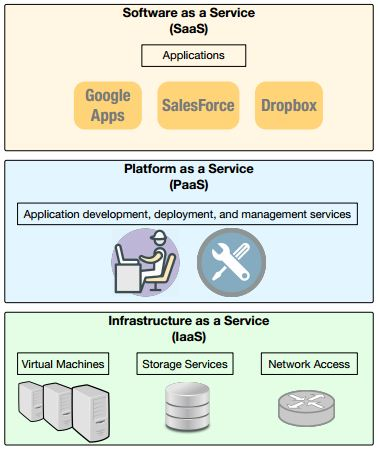
\includegraphics[width=190pt,height=240pt]{figures/cloud-computing.JPG}}\\
%		\caption[Cloud computing service offerings]{\footnotesize \textbf{{Cloud computing service offerings} }}
%\label{fig:ccs}
%\end{center}		
%\end{figure}

\subsection{Versions of Angular}
\hspace{0.2in}Early version of Angular framework was called as AngularJS. Angular 2+ versions are simply called as Angular. It is a completely rewritten version of AngularJS \cite{rewritten}. In this work, Angular refers to the Angular 2+ versions, unless otherwise stated. 

\subsection{Differences in AngularJS and Angular 2+}
Differences between AngularJS and Angular  2+ have stated below.
 
\begin{itemize}
\item{\textbf{ Speed :}  Angular is much faster than AnguarJS. Boot time of Angular applications has been increased by at least 5 times \cite{faster}.}
\item{\textbf{ Architecture :} Angular does not use \$scope or controllers anymore, instead it uses a hierarchy of components. }
\item{\textbf{ Mobile development :} Angular mainly focuses on  performance issues which are issential for running app on a Mobile Platform. }
\item{\textbf{ Modularity :} The core functionality of Angular has been moved to modules, producing a faster, lighter core. }
\item{\textbf{ Language :} Angular uses typescript to write applications, where as AngularJS uses javascript. TypeScript is a superset of JavaScript.}
\item{\textbf{ Improved dependency injection :} Angular used a new Improved Dependacy Injection techniques. }
\end{itemize}



%%::::::::::::::::::::::::::::::::::::::::::::::::::::::::::::::::::::::::::::::::::::::::::::::::::::::::::::::::::::::::::::::
\section{REST}

\hspace*{0.2in}REpresentational State Transfer (REST) \cite{rest} is a set of principles that describes how resources on a server machine are addressed and accessed by  another machine on the same network. The resources (or also called as Web Services) exposed via REST are often called RESTful Web Services. 

Characterization of RESTful Web Services can be given as :
\begin{itemize}
\item{ RESTful Web Services should be stateless \cite{stateless}. }
\item{ Every resource should be uniquly addressable. }
\item{ Access resources over HTTP commands of GET, PUT, DELETE, POST etc. }
\item{ Returned response should in XML or JSON. }
\end{itemize}

\hspace*{0.2in}In RESTful Web Services, every resource is given a URI (Uniform Resource Identifier). A resource can be a file, single record in the database, set of records, a table or the database itself etc. When this resource is requested by a client machine, it is converted into a uniform format (XML or JSON) before sending which can be understood by both machines.  RESTful Web Services are stateless \cite{stateless}. All the session information is stored only in the client machine. Each request from any client carries all the neccessary information to successfully complete the request.

\hspace*{0.2in}SOAP \cite{soap} is another standard as an alternavice for REST but with some differences. SOAP-based Web Services have an official standard, but REST-based Web Services don't.  SOAP is a protocol, but REST is an architectural style. REST is not really a standard but it makes use of other standards such as HTTP, XML, URI, JSON etc.

\subsection{REST Semantics}

\hspace*{0.2in}A RESTful API ( Application Programming Interface ) is simply a collection of URIs ( Uniform Resource Indentifiers ), all HTTP requests to these URIs and some JSON ( XML is also preferred as much as JSON ) representations of resources. These URIs should follow a principal that adheres to REST. Each resource on the server has its own URI or we can also call it an address.

\hspace*{0.2in}For resources residing on the server, nouns should be used as opposed to verbs which describes actions. A RESTful URI should refer to a resource that is a thing instead of referring to an action\cite{restnaming}.

\hspace*{0.2in}Some example of the server resources are given as follows:
\begin{itemize}
\item Users of the bulletin board system.
\item A list of courses taught by a professor.
\item A user's posts over a period of time.
\item An article about global warming.
\end{itemize}

\hspace*{0.2in}Each resource on the server exposing RESTful Web Services will have at least one URI to identify that resource. URIs should follow a predictable, hierarchical structure to enhance understandability and, therefore, usability. This is not a REST rule or constraint, but it keeps the API look better and easier to follow\cite{restnaming}.


Below some examples explained how one should define URIs for server resources:\\

To create a new student on the server:\\
\begin{lstlisting}[language=command]
	POST http://www.example.com/students\\
\end{lstlisting}

To read a student with Student ID 33:\\
GET http://www.example.com/students/33 \\
The same URI can be used for PUT and DELETE, to update and delete, respectively.\\

Here is an example URIs for courses:\\
POST http://www.example.com/courses for creating a new course.\\

GET|PUT|DELETE http://www.example.com/courses/62\\
for reading, updating, deleting course 62, respectively.\\

What if there is a need to apply to new course for a student? One option can be: \\
POST http://www.example.com/courses \\
And that could work to add a course, but it looks like it is outside the context of a student.\\

Because we want to add a new course for a student, this URI doesnt look , as it should be. It could be argued that the following URI would offer better clarity: \\
POST http://www.example.com/students/33/courses \\
Now we know we're adding a new course for Student ID 33.\\

Now what would the following return?\\
GET http://www.example.com/students/33/courses\\
Probably a list of courses for student id 33 has has enrolled. Note: we may choose to not support DELETE or PUT for that url since it's operating on a collection.\\


\section{HTTP}


\hspace*{0.2in}HTTP is very popular Request–-Response protocol in the client–server model in a network. A browser software, for example, could be the client in this model and an application running on a other machine having a website may be the server in this model. The client makes an HTTP request to the server. The server  provides resources such as HTML files and other many types of content, or it performs other tasks on behalf of the client machine, returns a response message to the client. The response received from server contains status information about the sent request and possibly could also contain requested content in its message body.

\subsection{HTTP Methods}

HTTP protocol defines `methods' (sometimes also called as verbs) to indicate the required action that needs to be performed on the identified resource. This resource represents, whether existing data or data that is generated on the fly, relies on the implementation of the server. 

\begin{enumerate}
\item \textbf{GET : } The HTTP GET method is used to read a resource residing on a server. In a successful request, GET returns a response in XML/JSON and an HTTP response code of 200. In case if an error occures , it returns code 4** or 5**, but mostly returns a 404 (404 is a NOT FOUND) or 400 (400 is a BAD REQUEST).

\hspace*{0.2in}GET requests are used only to read resources and not to change them. So, when used this way (i.e without modifiying anything on the server ), they are considered safe. They (requests) can be called without any risk of data modification (or data corruption)—calling it once has the similar effect as calling it 100 times, or none at all. Also, GET is a idempotent request, which means that making multiple similar requests will have the same result as a single very first  request.

Examples:\\
GET http://www.example.com/students/123\\
GET http://www.example.com/students/123/courses\\

\item \textbf{HEAD : } The HEAD method in the HTTP protocol desires for a response similar to that of a GET request, but no response body should be there. This is  very useful for fetching metadata specified in response headers, without having to transport the full content that comes with that request.

\item \textbf{POST : } The POST method in HTTP is mostly used to create new resources on the server. On successful creation of a resourse, it return HTTP response status 201, returning a Location header with a link to the just created resource with the 201 response status.

POST method is neither safe nor idempotent. It is desirable only for non-idempotent resource requests. Making two similar POST requests will mostly result in two resources containing the same type data.

Examples:\\
POST http://www.example.com/students\\
POST http://www.example.com/students/123/courses\\

\item \textbf{PUT : } PUT is used to update the resources residing on server, PUT-ing to a known resource URI with the request body containing the newly-updated resource. PUT can also be used to create new resources, but it is not recommanded. Also, use POST to create new resources and provide the client-defined ID in the body.

\hspace*{0.2in}On successful update operation, it should return 200 status code (or 204 if not returning any content in the body) from a PUT. If PUT used to create, should return HTTP status code 201 on successful creation of the resource. A body in the response is optional. It is optional to return a link in the location header in the creation case since the client already set the resource ID.

\hspace*{0.2in}PUT method is not safe, means it modifies a resource (or creates) state on the server, but it is idempotent. If you create or update a resource residing on the server using PUT method and then make that same request again, the resource is still there and also has the same state as it did with the very first request. If calling PUT on a resource increments a counter  value within the resource residing on the server, the call is no longer said to be idempotent. Many times it happens and it may be enough to document that the call is not idempotent. However, it's recommended to keep PUT requests idempotent.

Examples:\\
PUT http://www.example.com/students/123\\
PUT http://www.example.com/students/123/courses/987\\


\item \textbf{DELETE : } DELETE method in the HTTP protocol is used to delete a resource which is indentified by a URI address. On successful deletion of the resource, it returns HTTP status code 200 ( also called as OK response) with a response body, with a possible wrapped response. Either that or return HTTP status code 204 (called as NO CONTENT) without any response body in the reply. A 204 status code with no body, or the JSON-style response and HTTP status 200 are the recommended responses in this case.

\hspace*{0.2in}DELETE operations are idempotent operations. If you DELETE a resource residing on the server, it's will be removed, if access is granted. Calling DELETE multiple times on that resource ends up the same one: the resource is deleted. If calling DELETE , decrements a counter value, the DELETE call is no longer remains idempotent. Using POST for non-idempotent resource requests is desired and adheres to quality.

\hspace*{0.2in} Calling DELETE method on a resource, more than once will often return a 404 (also called NOT FOUND) since it was already deleted and so it is no longer available to delete. It just no longer exists. This makes DELETE operations no longer idempotent, but the end-state of the resource remains the same. Returning a 404 is ok and communicates well the status code of the request.

Examples:\\
DELETE http://www.example.com/students/123\\
DELETE http://www.example.com/students/123/courses\\


\item \textbf{PATCH : } PATCH is mostly be used for partially modifying resources residing on the server. The PATCH request only needs to contain the changes to the resource, it does not need the complete resource. This is similar to PUT, but the body of the request contains a set of operation that describe how a resource currently residing on the server should be modified to produce a new version of the resource. 

\hspace*{0.2in}PATCH method is neither safe nor idempotent operation. But a PATCH method request can be made in such a way that it looks idempotent, it also helps to  prevent bad outputs that come from collisions between two PATCH requests on the same resource at the same time. Collisions from many PATCH requests may be a lot more dangerous than PUT collisions because some patch formats need to operate from a known base-point. Clients using this kind of patch application hould be using a conditional request such that the request will be failed completely if the resource has been updated since the time that client last accessed the resource. For example, the client can make a use of ETag in an If-Match header on the PATCH request made to the server.

Examples:\\
PATCH http://www.example.com/students/123\\
PATCH http://www.example.com/students/123/courses/987\\

\end{enumerate}

%%::::::::::::::::::::::::::::::::::::::::::::::::::::::::::::::::::::::::::::::::::::::::::::::::::::::::::::::::::::::::::::::
\section{Observables}

\hspace*{0.2in}Observable are a very integral part of Angular. It  is not just specific to  Angular, but it is a popular standard used to manage asyncronous data. Observables allow a continuous stream of communication in which multiple data values can be sent over time. We get a pattern of processing the data by using operations similar to array operations to parse, modify. Angular framework makes use of observables broadly. Mostly used in the HTTP service and the event system of Angular.
	
	
\hspace*{0.2in}In an ordinary method call (which are synchronous), something like this happens:
\begin{enumerate}
\item Call a method.
\item Wait for the method to finish.
\item Store the return value from that method in a variable.
\item Use that variable and its new value to do something useful.
\end{enumerate}

\hspace*{0.2in}In the asynchronous model the flow goes more like this:
\begin{enumerate}
\item Define a method that does some work and returns a value from the asynchronous call
\item Define this asynchronous call as an Observable.
\item Subscribe to this Obervable and provide a method to be called.
\item Continue processing other things; whenever the call returns, the provided method will begin to operate on its return value or values -- the items emitted by the Observable.
\end{enumerate}


In many programming tasks, you more or less expect that the instructions (programs) you write and implement will execute and complete incrementally, one by one, in the order as you have written them. But in some cases, many instructions might execute in parallel and their results are captured afterwards, in random order, by “observers.” Rather than calling a function, you define a technique for fetching and transforming the data, in the form of an “Observable,” and then subscribe to it.

An advantage of this technique is when you have a lot  of tasks that are  independent of each other, you can start them all at the same time rather than waiting for each one to complete before starting the another one. This way your entire all of your tasks only takes as long to complete as the longest task among all tasks.



%%::::::::::::::::::::::::::::::::::::::::::::::::::::::::::::::::::::::::::::::::::::::::::::::::::::::::::::::::::::::::::::::
\section{Data Formats used }

\hspace*{0.2in}JSON, or JavaScript Object Notation, is a minimal, readable format for structuring data. It is used mainly to transmit data between a server and a client, as an alternative to XML. 
		
\hspace*{0.2in}It is a very common data format used for asynchronous client/server communication, including as a replacement for XML in some AJAX-style systems. JSON is a language-independent data format. It was derived from JavaScript, but as of year 2017 many programming languages include code to generate and parse JSON-format data. The official Internet media type for JSON is `application/json'. JSON filenames use the extension `.json'.


\subsection{JSON}

\textbf{What is JSON?}\\
\hspace*{0.2in}JSON, or JavaScript Object Notation, is a minimal, readable format used for structuring data. It is used primarily to send data between a server and web application(or client), as an alternative to XML. 

\textbf{Keys and Values}\\

The two primary properties that are part of JSON are keys and values. 

Key: A key is always a string specified in quotation marks.
Value: A value can be a string, number, boolean value (true or false), array, or object.
Key/Value Pair: A key value pair has a specific syntax, with the key then a colon followed by the value. Key/value pairs are separated by using a comma.
Let's take one line example of JSON and identify each part of the code.

"foo" : "bar"
This example is a key/value pair. The key is "foo" and the value is "bar".

\textbf{Types of Values}\\

Array: An associative array of values.
Boolean: True or false.
Number: An integer.
Object: An associative array of key/value pairs.
String: Zero or more text characters which mostly form a word.

\textbf{Arrays}\\

Array can be used as value in key/value pairs if JSON object. Array is represented by a square brackets, within it all values of array separated by comma.

"foo" : {
  "bar" : "Hello",
  "baz" : [ "quuz", "norf" ]
}

\textbf{Objects}\\

An object is specified by curly brackets. Everything inside of that curly brackets is part of that object. So that means "foo" and the corresponding object are a key/value pair.

"foo" : {
  "bar" : "Hello"
}\\
The key/value pair "bar" : "Hello" is nested inside the key/value pair "foo" : { ... }. \\
That's an example of a hierarchy in JSON data.

